\chapter{Grundlagen}
\label{Grundlagen}
Im Rahmen dieser Masterarbeit werden mehrere Softwarepakete und bereits bestehende Programme verwendet. Nachfolgend werden die wichtigsten Programme erläutert.
	\section{Docker}
	\label{Grundlagen:Docker}
		Docker bietet die Möglichkeit Anwendungen auf einem System zu isolieren und Strukturieren.
		Hiermit lassen sich einzelne Programme, oder zum Zeitpunkt der Containererstellung festgelegte Prozesse kapseln, in einen Container überführen und somit eine hochgradig agile Umgebung schaffen. \cite{dockerGetStarted}.
		In Abbildung \ref{fig:Grundlagen:Docker:DockerVsVM} wird der Unterschied zwischen einer \gls{VM} und der Docker Umgebung dargestellt.
		Es ist ersichtlich, dass innerhalb eines Docker Containers nicht von Grund auf das Betriebssystem ausgeführt werden muss. 
		Somit lassen sich die zur Verfügung stehenden Ressourcen des Host Computers effizienter bereitstellen.
		\begin{figure}[H]
			\centering
			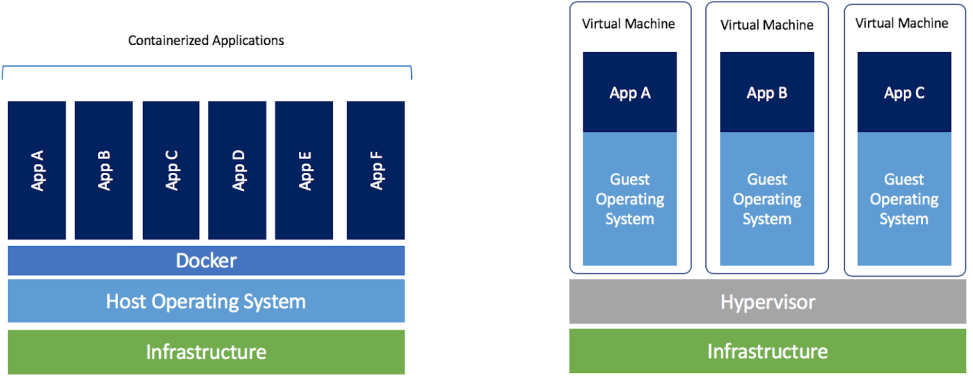
\includegraphics[width=\textwidth]{"Bilder/DockerVsVM.png"}
			\caption{Vergleich zwischen Docker und Virtuellen Maschinen. \cite{dockerVsVM}}
			\label{fig:Grundlagen:Docker:DockerVsVM}					
		\end{figure}
		Um tiefer ins Detail zu gehen, ist die Erläuterung der Begriffe Image, Container, Dockerfile und Docker-Compose notwendig.
		\paragraph{Image}
			Ein Docker-Image ist ein Speicherabbild eines Containers. 
			Das Image besteht aus mehreren Layern, die schreibgeschützt sind.
			Images können manuell erstellt werden, oder mit Verwendung eines dockerfiles automatisiert kompilliert werden.
			
		\paragraph{Container}
			Ein Container ist die aktive ausgeführte Instanz eines Images.
			Es läuft immer ein Prozess innerhalb des Containers.
			Somit wird ein Container beendet, sobald er kein Programm ausführt oder das Programm mit seinem Auftrag fertig ist.
			
		\paragraph{Dockerfile}
			Ein Dockerfile ist eine Textdatei mit Anweisungen zum erstellen eines Containers.
			Jeder Schritt erstellt einen neuen Layer, der dem Image hinzugefügt wird.
			Mit einem Dockerfile lässt sich das erstellen von Images automatisieren.
		
		\paragraph{Docker-Compose}
			Mit Docker-Compose lassen sich die Startparameter eines Containers in einer .yaml -Datei festlegen.
			Es lassen sich mehrere Docker-Container gleichzeitig starten, sowie umfangreiche Einstellungen bei dem Start des Containers treffen.
		
		\subsection{Netzwerke}
		\label{Grundlagen:Docker:Netzwerke}
			Docker bietet auch die Netzwerkkapselung für die Container an.
			Somit lässt sich das Netzwerk eines Containers von dem Rest des Systems oder anderen Containern trennen.
			Es können auch eigene Netzwerke definiert werden, um mehrere Container miteinander Kommunizieren zu lassen.
			Sie spannen so ein eigenes Netzwerk auf, was vergleichbar mit einem lokalen Netzwerk ist.
			Zwei Netzwerktypen die Docker anbietet, werden nachfolgend erläutert.
			\paragraph{Bridged}
				Das Bridged Netzwerk kapselt das Netzwerk des Containers von dem des Host Systems, bietet aber noch eine Netzwerk-Brücke, damit der Container Teilnehmer in höherliegenden Netzen erreichen kann.
				Es lassen sich Ports des Host-Computers an einen Container weiterleiten, um so eine Erreichbarkeit des Containers aus einem höherliegendem Netz zu ermöglichen.
				
			\paragraph{Host}
				Die Netzwerkeinstellung Host verzichtet auf eine Kapselung der Netze.
				Hier verwendet der Container die IP Adresse des Host-Computers und ist entsprechend teil des Host-Netzes.
				Für weitere Teilnehmer des Netzwerkes, ist der Host-PC des Docker-Containers und der Container selbst, dasselbe Gerät.
				Eine Portweiterleitung zum ermöglichen von Diensten ist hier nicht notwendig.
				
			\subsection{Datenspeicherung}
			\label{Grundlagen:Docker:Datenspeicherung}
				Nach beenden des Containers werden die Daten, die während dem ausführen des Containers angefallen sind, gelöscht.
				Um eine Persistente Speicherung, zu ermöglichen, bietet Docker mehrere Möglichkeiten an, um über die Laufzeit des Containers hinaus Daten zu speichern, oder auch um auf Daten innerhalb des Containers zuzugreifen. 
				Nachfolgend werden die wichtigsten kurz vorgestellt.
				
				\begin{figure}[H]
					\centering
					% \input{"Bilder/tikz/Grundlagen/docker-types-of-mounts.tex"}
					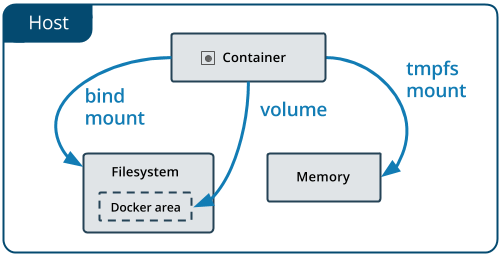
\includegraphics[width=0.70\textwidth]{"Bilder/DockerSpeichertypenpng.png"}
					\caption{Verschiedene Datenspeichermöglichkeiten. \cite{dockerStorage}}
					\label{fig:Grundlagen:Docker:Datenspeicherung}					
				\end{figure}
										
				\paragraph{Volumes}
					Volumes werden auf dem Dateisystem des Hosts gespeichert (In Linux unter \textit{/var/lib/docker/volumes/}).
					Ein Volume kann in mehrere Container eingebunden werden, dadurch ist eine containerübergreifende Dateiablage möglich.
					Volumes werden nicht automatisch gelöscht, sobald alle Container gestoppt sind, welches das Volume eingebunden hatten.
					Sie eignen sich am besten, um Daten Persistent zu speichern. \cite{dockerStorage}
				
				\paragraph{Bind mounts}
					Bind mounts können überall auf dem Hostsystem gespeichert sein.
					So können wichtige Systempfade (zum Beispiel \textit{/dev/}) dem Container zugänglich gemacht werden. \cite{dockerStorage}
				
				\paragraph{tmpfs mounts}
					Hier werden die Dateien nicht auf dem Dateisystem des Hosts gespeichert, sondern auf dem Arbeitsspeicher des System.
					Dadurch entsteht eine nicht persistente Datenspeicherung, um geheime Informationen zwischen Containern auszutauschen. \cite{dockerStorage}
					
				
	\section{Industrial Edge}
	\label{Grundlagen:IndustrialEdge}
		Industrial Edge ist eine Entwicklung von Siemens, die ermöglicht, im Prozess anfallende Daten bereits auf dem Gerät zu analysieren.
		Es wird lokales Engineering mit Cloud Engineering kombiniert. \cite{siemensIEM_gettingStarted}
		Dadurch werden unnötige Datentransporte zwischen dem Endgerät und Server vermieden und erst bereits aufbereitete Daten zum Server geschickt.
		Die Rechenlast fließt so vom Server in Richtung des Endgerätes.
		Hierfür werden Applikationen (Apps) bereitgestellt, die einen festen Funktionsumfang enthalten und mit der Industrial Edge Infrastruktur auf das jeweilige Endgerät (Edge Device) gespielt werden können.
		Diese Apps basieren auf der Docker Technologie.
		Industiral Edge ermöglicht die zentrale Verwaltung von
		In der nachfolgenden Abbildung \ref{fig:Grundlagen:IndustrialEdge:Ueberblick} ist eine typische Infrastruktur von dem obersten Server, bis zu den Endgeräten dargestellt, die im Nachfolgenden näher erläutert wird.
		\begin{figure}[h]
			\centering
			%\input{"Bilder/tikz/Grundlagen/industrial-edge-overwiev.tex"}
			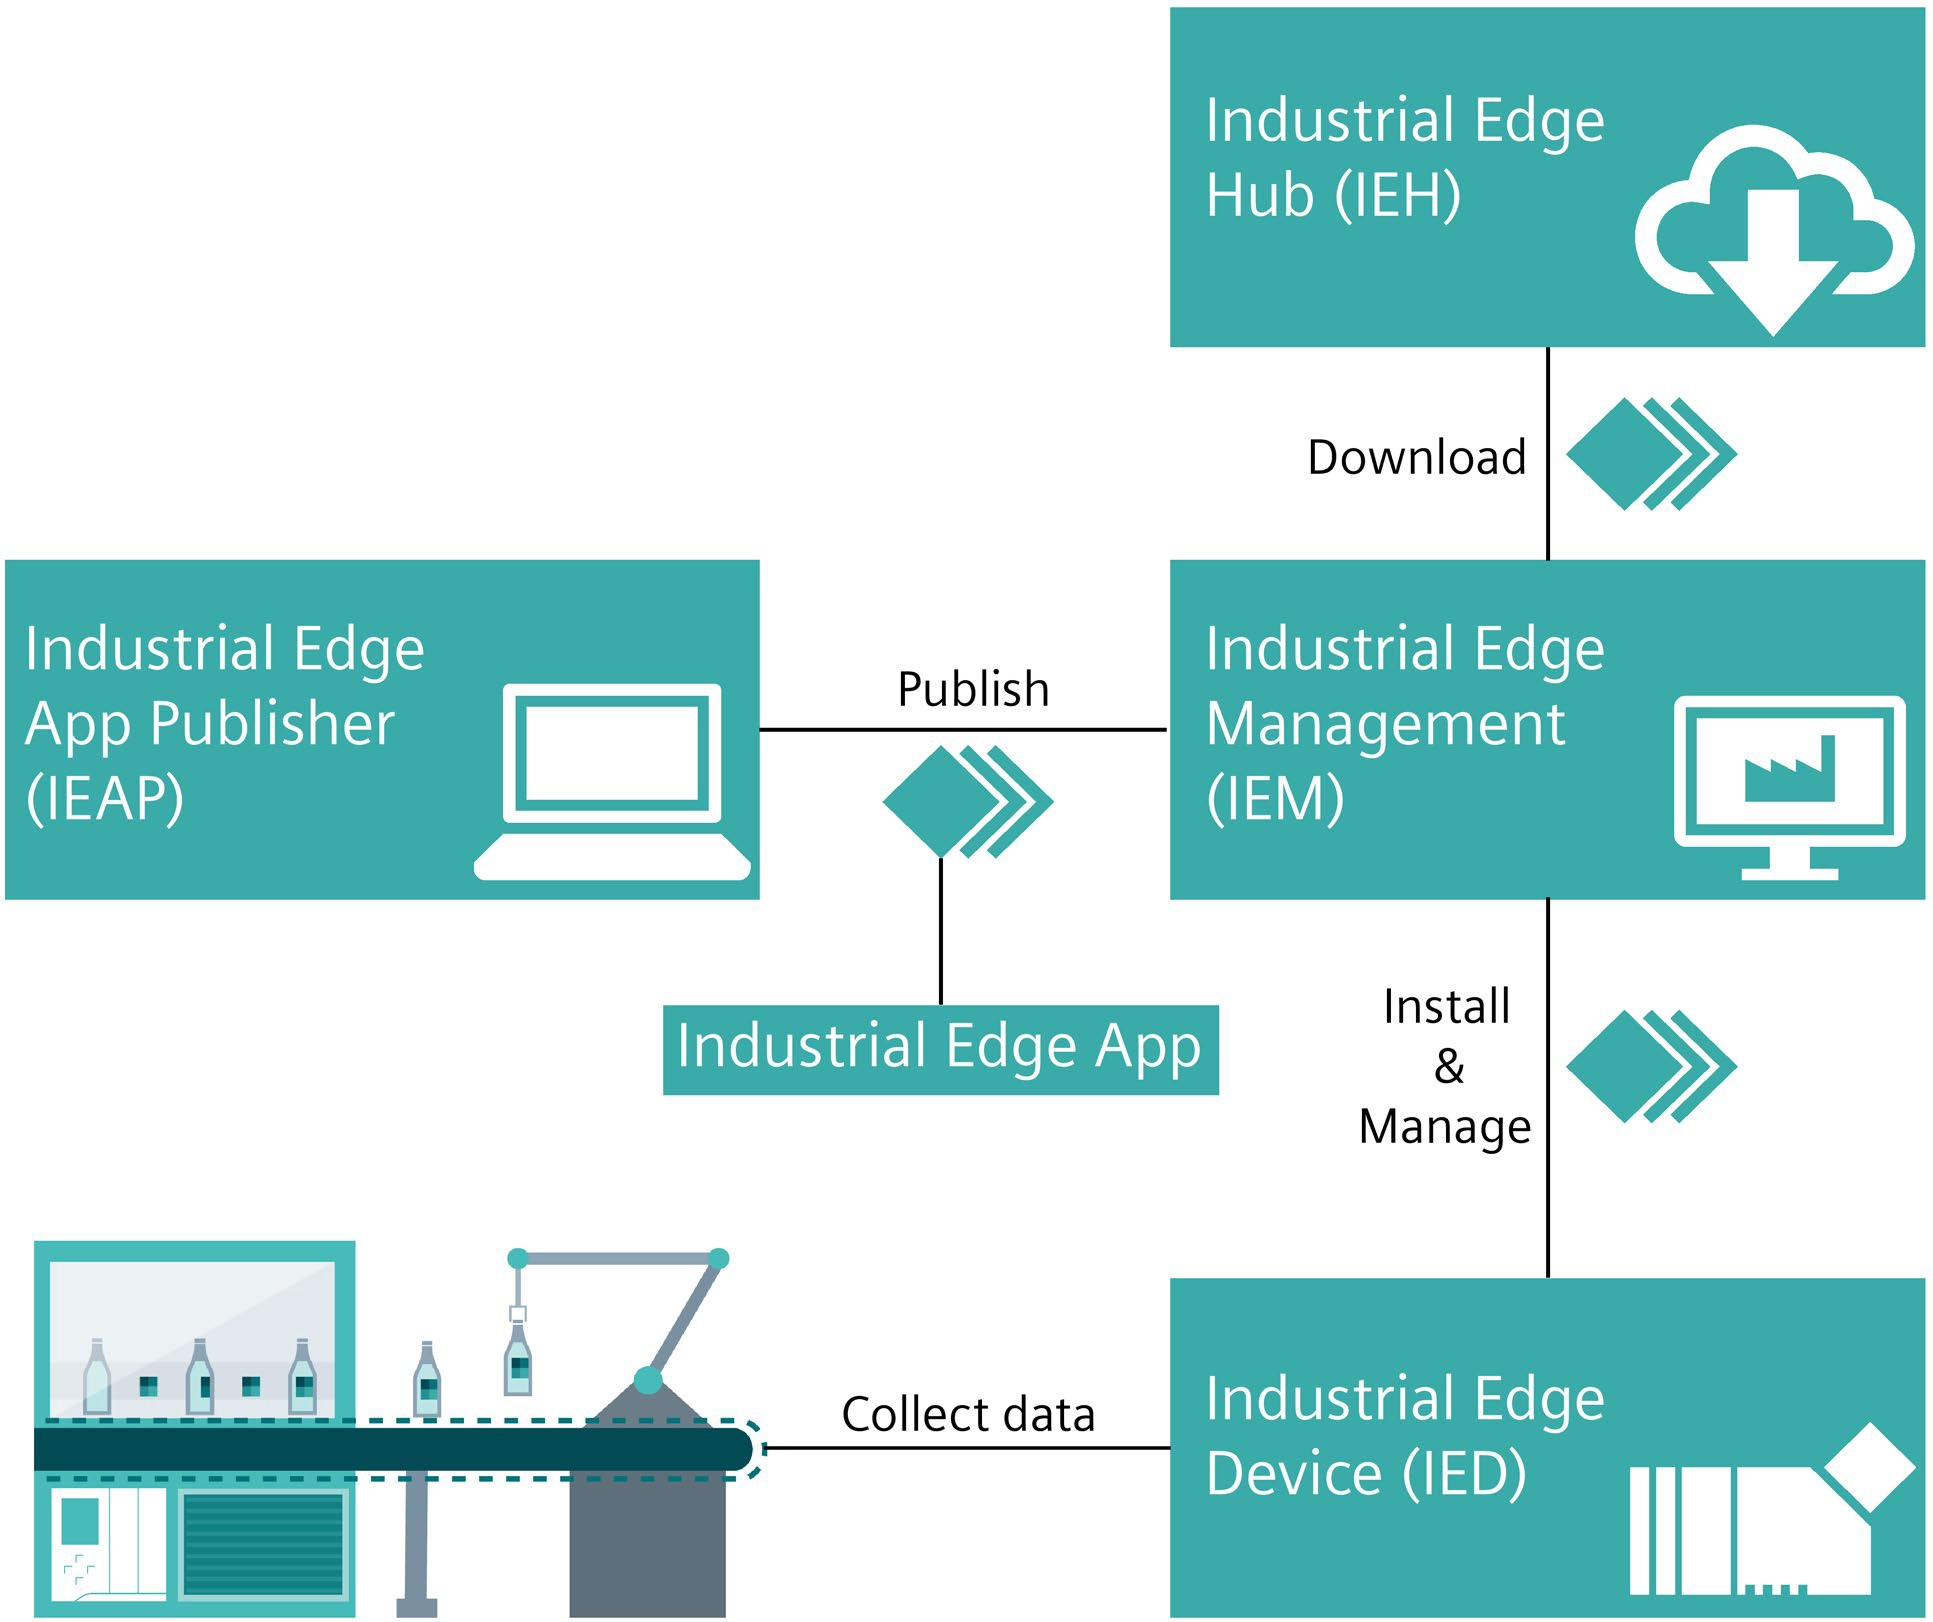
\includegraphics[width=0.70\textwidth]{"Bilder/Edge_uebersicht.jpg"}
			\caption{Überblick über Industrial Edge. \cite{siemensIEM_gettingStarted}}
			\label{fig:Grundlagen:IndustrialEdge:Ueberblick}					
		\end{figure}
	
		%- Management tool für Docker Container auf Geräten (Device)\\
		%- Graphen die das IE-Hub, IEM, Docker Device erklärt\\
			
		\paragraph{Industrial Edge Hub}
			Das \gls{IEH} ist die oberste, von Siemens bereitgestellte Serverebene.
			Hier bietet Siemens eigene entwickelte Applikationen an, die gegen eine Lizenzgebühr auf das \gls{IEM} geladen werden können.
			Von hier aus lassen sich ebenfalls benötigte Softwarepakete und Dokumentation herunterladen, die das Entwickeln von eigenen Apps und das Aufsetzen und betreiben von einem eigenen \gls{IEM} ermöglicht. \cite{siemensIEM_gettingStarted}
			
		\paragraph{Industrial Edge Management System}
			Das \gls{IEM} ist ein Server, welcher in einem Lokalen Netz selbstständig betrieben werden kann.
			Der Anwender hat hiermit die Möglichkeit, einen Server zu erstellen, damit z.B. sensible Daten, die zwischen dem Edge Device und dem \gls{IEM} ausgetauscht werden, nicht über das Internet transportiert werden müssen.
			Zudem lassen sich die Endgeräte über diesen Server verwalten, es können Apps sowie Softwareupdates aufgespielt werden, sowie lassen sich weitere Analysen durchführen.
			Eine selbst entwickelte App lässt sich auf das \gls{IEM} aufspielen, welches Diese wiederum an die Edge Devices verteilen kann.
			\cite{siemensIEM_gettingStarted}
			
		\paragraph{Industrial Edge App}
			Eine Edge App dient zur intelligenten Verarbeitung von Automatisierungsaufgaben. \cite{siemensIEM_gettingStarted}
			Neben den von Siemens im \gls{IEH} angebotenen Apps lassen sich auch eigene Applikationen entwickeln.
			Diese und eigene entwickelte Apps sind Docker basierte Images, welche auf dem \gls{IED} ausgeführt werden.
			Als oberste Beschreibungsebene wird eine docker-compose Datei angelegt, in welcher beschrieben wird, wie die docker Images zu starten sind, sowie welche Netzwerkkonfiguartion (Kapitel \ref{Grundlagen:Docker:Netzwerke}) und welche Art der Datenspeicherung (Kapitel \ref{Grundlagen:Docker:Datenspeicherung}) verwendet wird.
	
		\paragraph{Edge Device}
			Ein \gls{IED} führt die einzelnen Edge Apps aus. Sie können Automatisierungsdaten lokal speichern und nach Bedarf abrufen. 
			Ebenfalls lassen sich diese Daten an eine Cloud-Infrastruktur übermitteln. Ein \gls{IED} muss bei einem \gls{IEM} aktiviert werden.
			\cite{siemensIEM_gettingStarted}
			
		\paragraph{Industrial Edge Publisher}
			Der Industrial Edge Publishers ist ein Tool, mit dem Docker Images in Edge Apps überführt und in das \gls{IEM} hochgeladen werden.
			Es lassen sich ebenfalls bereits erstellte Apps verwalten, verändern oder löschen.
			\cite{siemensIE_App}

	
	\section{Simatic Automation Tool}
	\label{Grundlagen:SAT}
		Mit dem \gls{SAT} kann eine SPS konfiguriert werden.
		Dieses Tool steht für Windows sowie Linux mit deb oder rpm Paketverwaltung zur Verfügung. \cite{siemensSAT}
		Mit der Linux Version lässt sich die IP Adresse der SPS anpassen, ein bereits kompiliertes Programm downloaden, eine CPU in RUN oder STOP versetzen, eine CPU auf Werkseinstellung zurücksetzen, sowie die Firmware der SPS updaten\cite{siemensSAT_Online}. 
		Die Linux Version von \gls{SAT} stellt unter anderem folgende Befehle zur Verfügung:
		\begin{lstlisting}[caption={Beispielbefehle für SAT}, label={code:SATBeispiel}]
			transfer_sat -f /path/to/OMS.zip -i 123.231.123.3
			transfer_sat -c /path/to/OMS.zip
		\end{lstlisting}
		In Zeile eins des Listings \ref{code:SATBeispiel} wird das Kompilat welches in \lstinline|/path/to/OMS.zip| auf die SPS mit der IP Adresse \lstinline|123.231.123.3| geladen. 
		Voraussetzung ist, dass diese IP Adresse erreichbar ist.
		Mit dem Befehl in Zeile zwei lässt sich die angegebene Datei überprüfen.
		Anhand des Rückgabewerts lässt sich bestimmen, ob die angegebene Operation erfolgreich verlief.
		Hierbei wurde der für Linux etablierte Standard, dass ein Rückgabewert 0 einen Erfolg des Programms bestätigt, eingehalten.
		Weitere Fehlercodes sind unter anderem 100, der auf einen nicht erreichbaren Host hinweist, oder 103, welcher auf einen nicht erfolgreichen Download hinweist. \cite{siemensSAT}
					

	\section{ROS 2}
	\label{Grundlagen:ROS2}
		Ein asdfasdasd
		\cite{ros2Basic}
		\gls{ROS2}
	
	
	
		\subsection{Nachrichtentypen}
		\label{Grundlagen:ROS2:Nachrichtentypen}
			- Message (topics)\\
			- Service\\
			- Action
			
		\subsection{ROS 2-web Bridge}
		\label{Grundlagen:ROS2:2WebBridge}
			- Stellt einen websocket bereit, der mittels JSON requests verarbeitet. 
			- Basiert auf RclNodeJS, welches eine brücke zwischen javascript und ros2 bildet\\
			- Basiert auf NodeJS. NodeJs ist eine JavaScript Runtime, die JS Code serverseitig ausführen lässt.
			Das ist hier nicht weiter von relevanz.\\
			- Verwendet wird für die Anwendung ebenfalls roslibjs. Dies ist eine javascript bibliothek, welche in der html eingebunden wird. Sie stellt Befehle zum erstellen von ROS Subscriber/Publisher und Services bereit.\\
			
		\subsection{roslibjs}
		\label{Grundlagen:ROS2:RosLibJS}
	
	\section{DDS}
	\label{Grundlagen:DDS}
		- Grundlage für Kommunikation von ROS2\\
		- Realisiert die eigentliche Kommunikation\\
		- Wenn das hier geht, geht auch ROS2!
		- Verschiedene Systemanbieter, näher wird RTI und Fastrtps untersucht: https://ros.org/reps/rep-2000.html  (Beide TIER 1)
		
		ROS2 verwendet als Kommunikationsschnittstelle DDS.
		DDS funktioniert gut in lokalen Netzwerken, sobald allerdings ein NAT-Router dazwischen ist, funktioniert der standardmäßige Discovery Mechanismus nicht.
		Da das Ziel eine Edge Applikation ist, soll das Verhalten von DDS in der Docker Umgebung, bzw. in unterschiedlichen Netzwerken untersucht werden.
	
	\section{OpenController2}
	\label{Grundlagen:OpenController2}
		- Das ist ja meine zielhardware\\
		- Aktueller AGV läuft damit\\
		
	\section{TIA Openess}
	\label{Grundlagen:Fusionierung}
		- Lauras BA Vorstellen\\
		
		
		
